\documentclass[11pt,a4paper]{article}
\usepackage[utf8]{inputenc}
\usepackage[T1]{fontenc}
\usepackage[french]{babel}
\usepackage{geometry}
\geometry{margin=2.5cm}
\usepackage{graphicx}
\usepackage{float}
\usepackage{verbatim}
\usepackage{caption}
\renewcommand{\contentsname}{Sommaire}
\setlength{\parskip}{0.5em}
\setlength{\parindent}{0pt}

\title{Projet TND --- Analyse des céréales}
\author{Binôme 5}
\date{2025--2026}

\begin{document}
\maketitle
\tableofcontents
\newpage

\section{Introduction}

Ce rapport porte sur 77 céréales de petit-déjeuner vendues aux États-Unis. On cherche à savoir comment elles se différencient sur le plan nutritionnel et s'il existe des groupes homogènes parmi elles.

Chaque céréale est décrite par 16 variables : sa composition nutritionnelle (calories, protéines, graisses, etc.), son conditionnement (poids, taille de portion) et quelques métadonnées (fabricant, type de consommation, note de satisfaction). Ces variables sont exprimées dans des unités sans rapport entre elles (Kcal, grammes, milligrammes, note sur 100). Ce point n'est pas anodin : il pèse directement sur le choix de la méthode.

On a retenu une ACP normée pour réduire la dimension et lire les liens entre variables, puis deux classifications (CAH et K-means) pour regrouper les céréales par profil nutritionnel. Les deux méthodes de classification servent aussi à se contrôler l'une l'autre.

\section{Description des données}

\subsection{Présentation du jeu de données}

Le fichier \texttt{276-cereals.txt} (le « 276 » est un simple identifiant de fichier, pas un effectif) contient 77 céréales et 16 variables. On les répartit en trois rôles :

\begin{itemize}
\item \textbf{Identifiant} : NAME, le nom de la céréale.
\item \textbf{Variables qualitatives} : MANUF (fabricant, 7 modalités : A, G, K, N, P, Q, R) et TYPE (C = froide, H = chaude).
\item \textbf{Variables quantitatives} (13) : CALORIES, PROTEIN, FAT, SODIUM, FIBER, CARBO, SUGARS, POTASS, VITAMINS, SHELF, WEIGHT, CUPS, RATING.
\end{itemize}

Le jeu est déséquilibré sur deux points. Côté type, 74 céréales froides pour seulement 3 chaudes. Côté fabricant, Kellogg's (23) et General Mills (22) représentent à eux deux près de 60\,\% des produits.

\subsection{Prétraitement}

Quelques cases valent -1 dans le fichier d'origine. Une teneur nutritionnelle négative n'a pas de sens : ce sont des valeurs manquantes déguisées. Il y en a 4 en tout, sur POTASS (2), CARBO (1) et SUGARS (1).

On les remplace par la médiane de leur variable plutôt que par la moyenne. FIBER et POTASS ont des distributions très étirées vers la droite ; sur ce genre de variable la médiane bouge beaucoup moins que la moyenne, et l'imputation reste donc raisonnable.

\subsection{Rôles des variables pour l'ACP}

Neuf variables servent d'actives, celles qui décrivent la composition nutritionnelle proprement dite : CALORIES, PROTEIN, FAT, SODIUM, FIBER, CARBO, SUGARS, POTASS et VITAMINS.

SHELF, WEIGHT, CUPS et RATING passent en supplémentaires quantitatives : elles ne construisent pas les axes mais on les projette ensuite pour les situer. WEIGHT et CUPS décrivent l'emballage, pas le contenu. RATING est une note déjà calculée par Consumer Reports : la garder en actif reviendrait à mélanger une synthèse avec ses propres ingrédients, alors qu'en supplémentaire elle devient un test (l'ACP retrouve-t-elle ce que mesure cette note ?). MANUF et TYPE complètent comme supplémentaires qualitatives.

\section{Statistiques descriptives}

\subsection{Analyse univariée}

\begin{table}[H]
\centering
\caption{Statistiques des variables actives}
\begin{tabular}{lrrrr}
\hline
 & Moyenne & Médiane & Écart-type & Skewness \\
\hline
CALORIES & 106.9 & 110.0 & 19.5 & -0.44 \\
PROTEIN  & 2.5   & 3.0   & 1.1  & 0.73 \\
FAT      & 1.0   & 1.0   & 1.0  & 1.14 \\
SODIUM   & 159.7 & 180.0 & 83.8 & -0.56 \\
FIBER    & 2.2   & 2.0   & 2.4  & 2.38 \\
CARBO    & 14.8  & 14.5  & 3.9  & 0.11 \\
SUGARS   & 7.0   & 7.0   & 4.3  & 0.04 \\
POTASS   & 98.4  & 90.0  & 69.5 & 1.40 \\
VITAMINS & 28.2  & 25.0  & 22.3 & 2.42 \\
\hline
\end{tabular}
\end{table}

Deux variables sortent du lot : FIBER (skewness 2.38) et VITAMINS (2.42) sont fortement étirées à droite. Autrement dit, la grande majorité des céréales en contiennent peu, et quelques produits très enrichis tirent la moyenne vers le haut. SUGARS, à l'inverse, est presque symétrique (0.04) : on trouve un peu de tout entre céréales peu et très sucrées.

\begin{figure}[H]
\centering
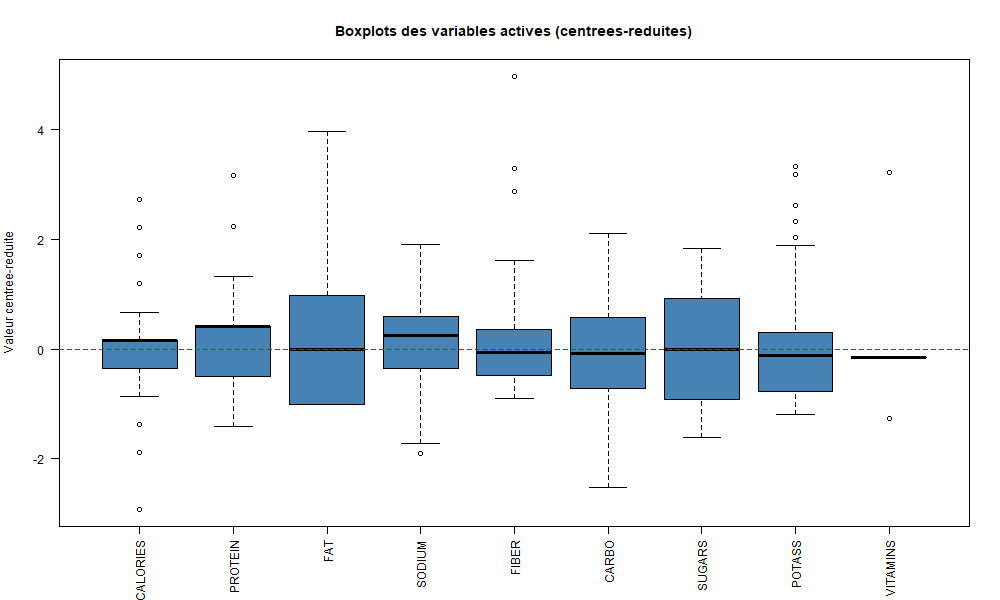
\includegraphics[width=0.78\textwidth]{output/figures/01_boxplots_actives.png}
\caption{Boxplots des variables actives (centrées-réduites)}
\end{figure}

Les boxplots confirment plusieurs points extrêmes : FIBER et POTASS pour les All-Bran, VITAMINS pour les céréales « Total » enrichies à 100\,\% des apports. On garde ces observations : ce sont de vrais produits du marché, atypiques mais réels, et les écarter biaiserait l'analyse.

\subsection{Analyse bivariée}

\begin{figure}[H]
\centering
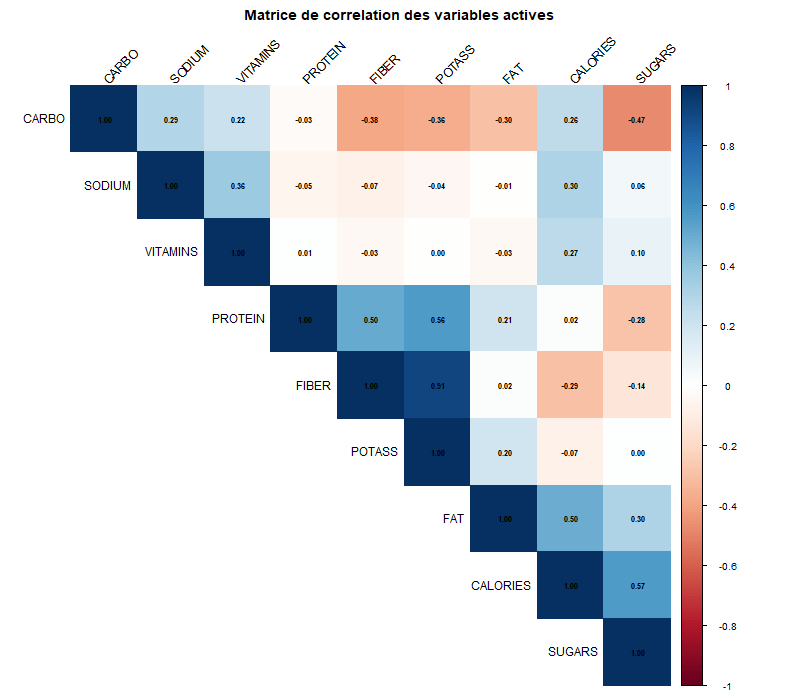
\includegraphics[width=0.66\textwidth]{output/figures/03_heatmap_correlation.png}
\caption{Matrice de corrélation des variables actives}
\end{figure}

La corrélation la plus forte relie FIBER et POTASS (r = 0.91). Rien d'étonnant : les céréales complètes, riches en fibres, gardent les minéraux du grain, dont le potassium. CALORIES suit SUGARS (0.57) et FAT (0.50), ce qui revient à dire que sucre et gras sont des sources de calories.

CARBO et SUGARS sont corrélées négativement (-0.47). Cela surprend au premier regard, mais c'est cohérent : dans une céréale, les sucres simples remplacent l'amidon plutôt qu'ils ne s'y ajoutent. Plus de sucre, donc moins de glucides complexes.

Ces dépendances justifient l'ACP. Les 9 variables ne sont pas indépendantes, et réduire la dimension permet de mieux voir la structure derrière ces corrélations.

\section{Analyse en composantes principales}

\subsection{Pourquoi une ACP normée}

Les unités n'ont rien de comparable. SODIUM a un écart-type de 84, POTASS de 69, FAT de 1. Une ACP non normée laisserait SODIUM et POTASS écraser les autres variables uniquement parce qu'elles sont mesurées dans de plus grands nombres. L'ACP normée travaille sur la matrice de corrélation, après centrage-réduction : chaque variable pèse alors le même poids, ce qui est ce qu'on veut ici.

\subsection{Valeurs propres et nombre d'axes}

\begin{figure}[H]
\centering
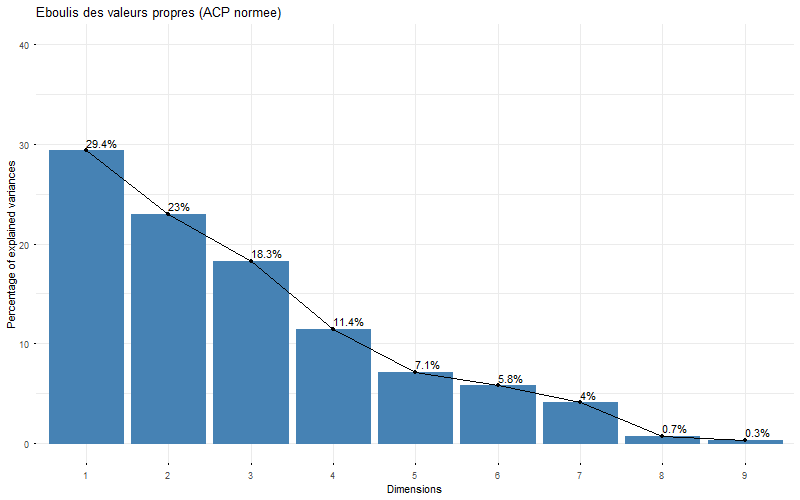
\includegraphics[width=0.6\textwidth]{output/figures/06_scree_plot.png}
\caption{Éboulis des valeurs propres}
\end{figure}

Le critère de Kaiser (valeurs propres > 1) retient 4 axes, soit 82.1\,\% de l'inertie. Les deux premiers en cumulent 52.4\,\%, ce qui reste correct pour 9 variables. L'éboulis ne montre pas de coude franc mais une décroissance régulière. On interprète le plan (1,2) en détail, sans oublier que les axes 3 et 4 portent encore de l'information utile (voir plus bas).

\subsection{Cercle des corrélations}

\begin{figure}[H]
\centering
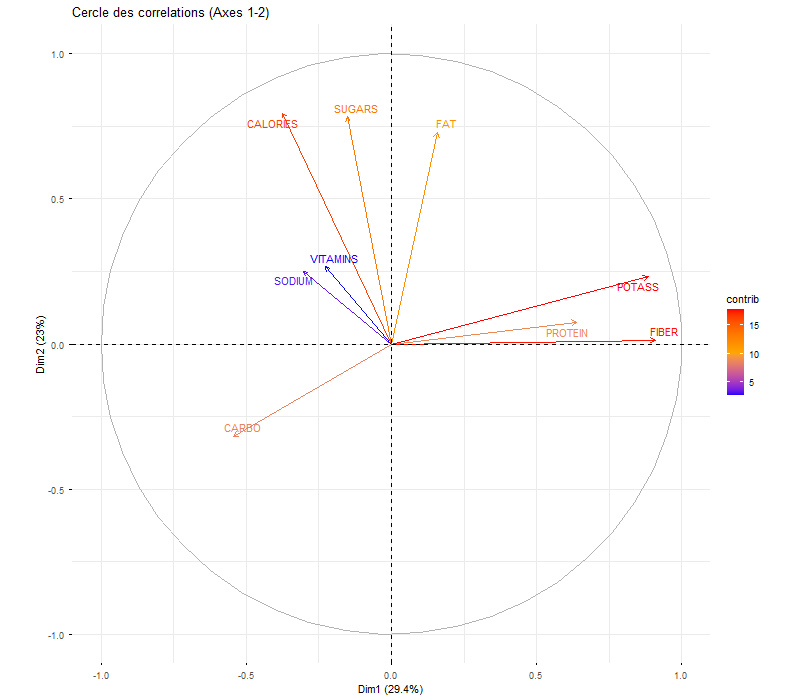
\includegraphics[width=0.66\textwidth]{output/figures/07_cercle_correlations_12.png}
\caption{Cercle des corrélations (axes 1-2)}
\end{figure}

L'axe 1 (29.4\,\%) est tiré par FIBER et POTASS du côté positif : c'est un gradient de richesse en fibres. À droite, les céréales complètes ; à gauche, les céréales raffinées qui en sont pauvres.

L'axe 2 (23.0\,\%) oppose CALORIES, FAT et SUGARS (en haut) à un pôle neutre (en bas). C'est un axe de densité calorique : plus on monte, plus la céréale est calorique, grasse et sucrée.

SODIUM et VITAMINS ont des vecteurs courts sur ce plan : ils y sont mal représentés. C'est attendu, ces deux variables s'expriment sur les axes suivants. L'axe 3 isole pour l'essentiel SODIUM (le sel ajouté, indépendant du profil fibres/sucre), et l'axe 4 VITAMINS (l'enrichissement artificiel, qui ne suit aucune autre variable nutritionnelle). Cela explique pourquoi le critère de Kaiser en garde 4 alors que le plan principal n'en montre que 2. Enfin, CARBO se place en bas à gauche, à l'opposé de SUGARS : on retrouve l'opposition amidon / sucres simples déjà vue dans les corrélations.

\subsection{Carte des individus et biplot}

\begin{figure}[H]
\centering
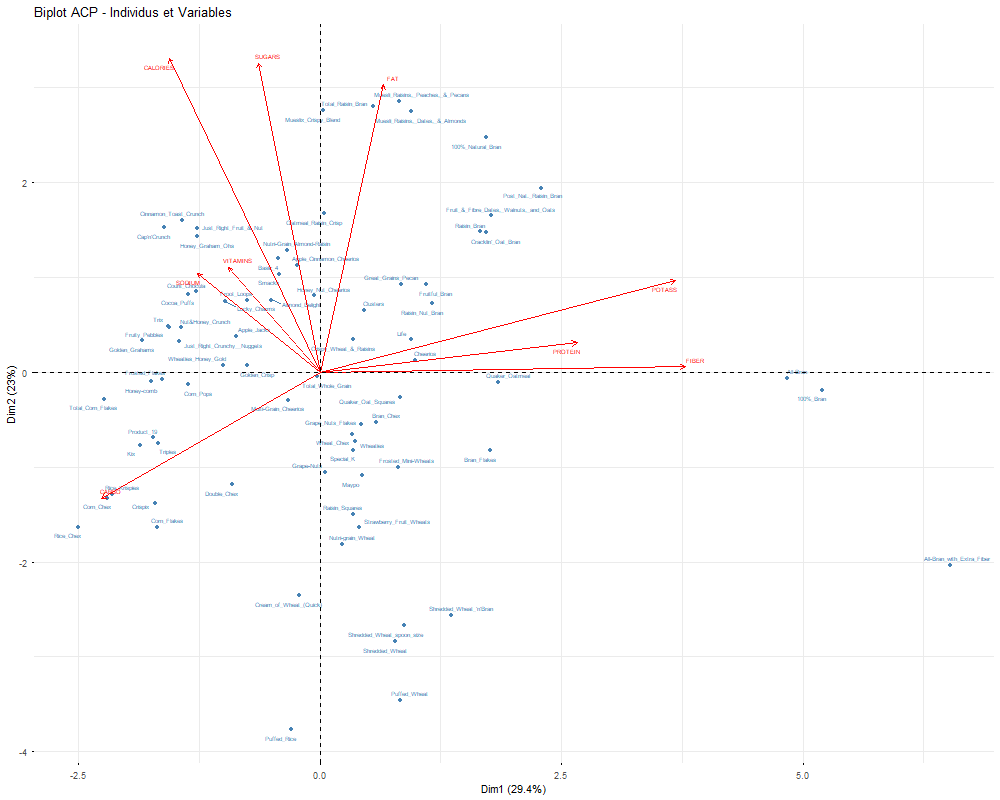
\includegraphics[width=0.76\textwidth]{output/figures/10_biplot.png}
\caption{Biplot --- individus et variables}
\end{figure}

Le biplot superpose céréales et variables. Les trois All-Bran (100\% Bran, All-Bran, All-Bran with Extra Fiber) sont seules tout à droite, du côté des fibres. À l'opposé, les céréales de riz ou de maïs (Rice Chex, Corn Chex) en sont pauvres. En haut, les céréales sucrées (Cap'n'Crunch, Froot Loops, Lucky Charms) se calent sur les vecteurs SUGARS et CALORIES. En bas, les peu caloriques comme Puffed Rice ou Shredded Wheat.

\subsection{Variables supplémentaires}

RATING se projette à +0.62 sur l'axe 1 et -0.72 sur l'axe 2. Traduction : les céréales bien notées sont riches en fibres et pauvres en calories et en sucre. La note de Consumer Reports recoupe donc de près la qualité nutritionnelle telle que la dessinent les deux premiers axes, alors qu'elle n'a pas servi à les construire.

Côté fabricants, Nabisco (N) tombe dans le quadrant « fibres élevées, peu calorique », ce qui colle à sa gamme Shredded Wheat. General Mills et Kellogg's restent au centre, avec des gammes plus larges. Les 3 céréales chaudes se détachent des froides, mais 3 individus ne permettent aucune conclusion solide.

\section{Classification}

\subsection{CAH --- méthode de Ward}

\begin{figure}[H]
\centering
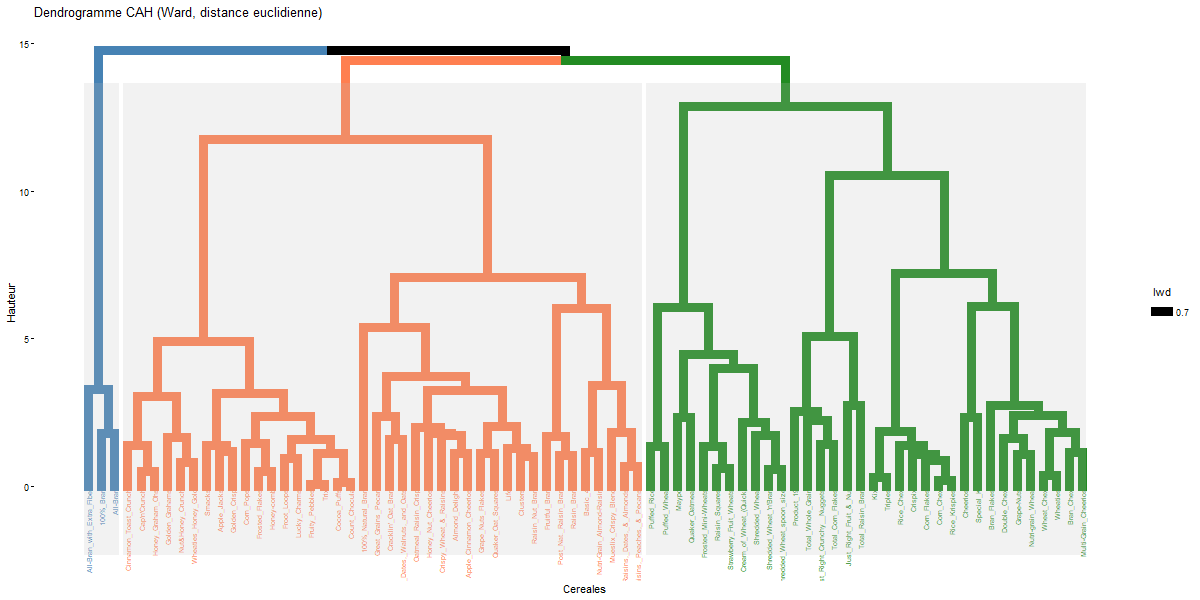
\includegraphics[width=0.9\textwidth]{output/figures/12_dendrogramme.png}
\caption{Dendrogramme (CAH, Ward, distance euclidienne)}
\end{figure}

La CAH utilise la distance euclidienne sur données centrées-réduites et le critère de Ward, qui minimise la hausse d'inertie intra-classe à chaque fusion. Ce critère va de pair avec la distance euclidienne et donne des classes de taille assez équilibrée.

Le dendrogramme penche pour 3 classes, avec un saut d'inertie net entre 3 et 2. La silhouette moyenne vaut 0.21 à k=3, ce qui est modeste. À k=2 elle monte à 0.45, donc plus propre, mais on perd alors le petit groupe très riche en fibres, qui est justement le plus intéressant. On garde k=3 en connaissance de cause.

\begin{figure}[H]
\centering
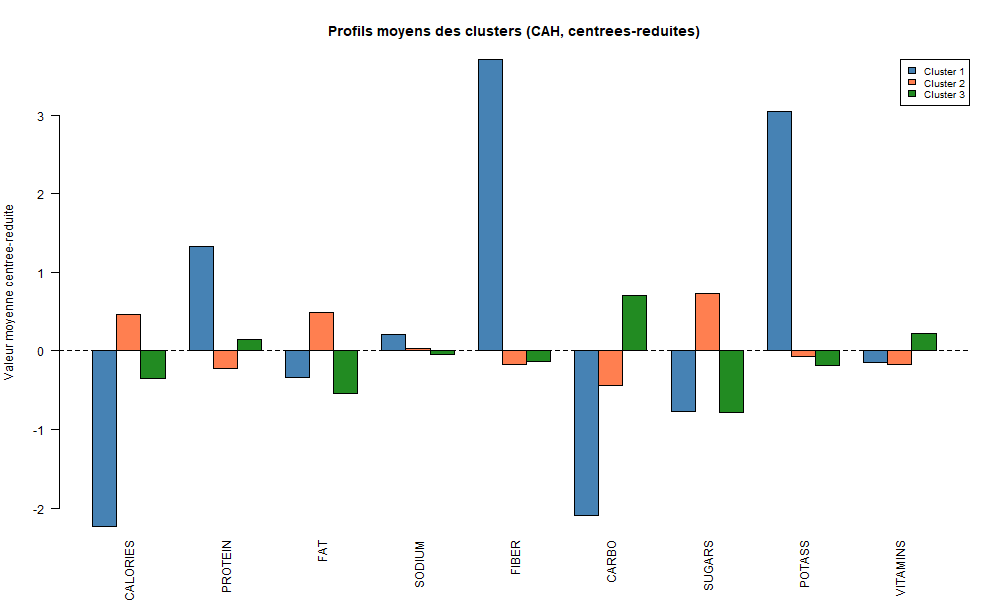
\includegraphics[width=0.78\textwidth]{output/figures/14_profils_cah.png}
\caption{Profils moyens des 3 clusters (CAH, données centrées-réduites)}
\end{figure}

Les trois classes (numérotation de la CAH) :

\begin{itemize}
\item \textbf{Cluster 1} (3 céréales) : profil haute fibre. FIBER et POTASS très élevés, CALORIES et CARBO bas. Ce sont les trois All-Bran.
\item \textbf{Cluster 2} (40 céréales) : profil sucré/calorique. SUGARS et CALORIES au-dessus de la moyenne, FIBER et CARBO en dessous.
\item \textbf{Cluster 3} (34 céréales) : profil modéré. Peu de sucre, peu de gras, CARBO élevé. Les classiques type Corn Flakes ou Rice Krispies.
\end{itemize}

Le cluster 1 ne pèse que 3 individus, ce qui le rend fragile. Ce sont au fond des points extrêmes, pas un « type » commercial de céréale. Sa séparation reste toutefois nette et se reproduit d'une méthode à l'autre. Pour vérifier qu'il ne déforme pas le reste, on a refait la CAH sans ces 3 céréales : la frontière entre le groupe sucré et le groupe modéré ne bouge presque pas. Le découpage principal ne dépend donc pas de ces outliers.

\subsection{K-means}

K-means tourne avec le même k=3 pour pouvoir comparer. On met \texttt{nstart=25} pour limiter l'effet du tirage initial, l'algorithme étant non déterministe contrairement à la CAH.

\begin{figure}[H]
\centering
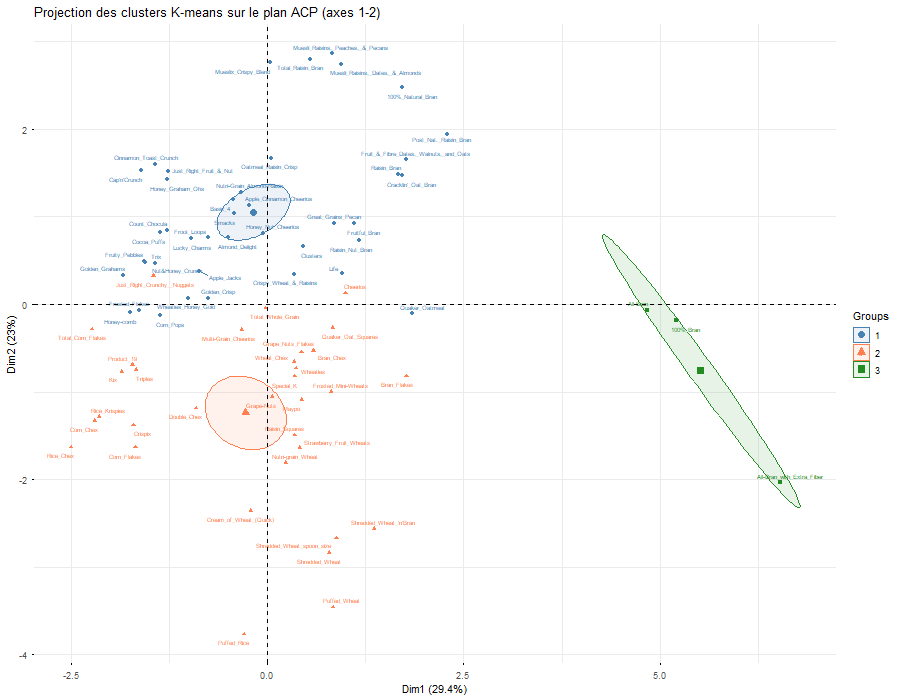
\includegraphics[width=0.78\textwidth]{output/figures/19_acp_clusters_kmeans.png}
\caption{Projection des clusters K-means sur le plan ACP}
\end{figure}

Les classes K-means ressemblent beaucoup à celles de la CAH. Sur le plan ACP, la séparation est lisible : le groupe haute fibre est isolé à droite, le groupe sucré en haut, le groupe modéré en bas à gauche.

\subsection{Comparaison CAH / K-means}

\begin{figure}[H]
\centering
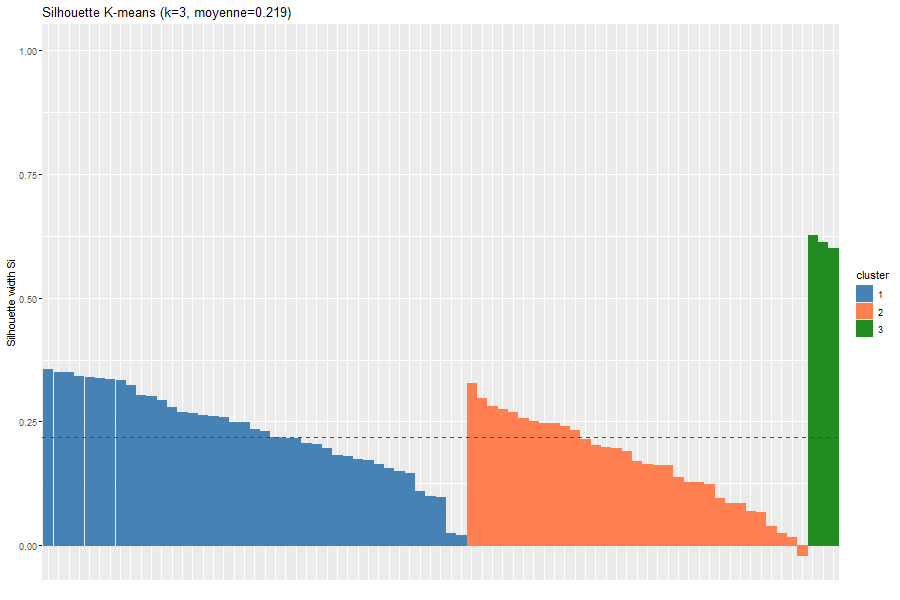
\includegraphics[width=0.66\textwidth]{output/figures/21_silhouette_kmeans.png}
\caption{Silhouette des clusters K-means}
\end{figure}

\textbf{Un point d'attention sur la numérotation.} Les numéros de clusters sont arbitraires et ne coïncident pas entre les deux méthodes. Le groupe haute fibre est le cluster 1 pour la CAH mais le cluster 3 pour le K-means ; le groupe sucré et le groupe modéré sont eux aussi renumérotés. C'est normal (aucune des deux méthodes n'impose d'ordre) mais il faut en tenir compte en lisant les figures, où l'on raisonne par profil et non par numéro.

L'indice de Rand entre les deux partitions vaut 0.882 et la pureté 0.935 : environ 94\,\% des céréales tombent dans le même groupe d'une méthode à l'autre. Les écarts portent sur des céréales à la limite entre profil sucré et profil modéré, ce qui est logique : cette frontière est moins tranchée que celle qui isole les fibres.

\begin{figure}[H]
\centering
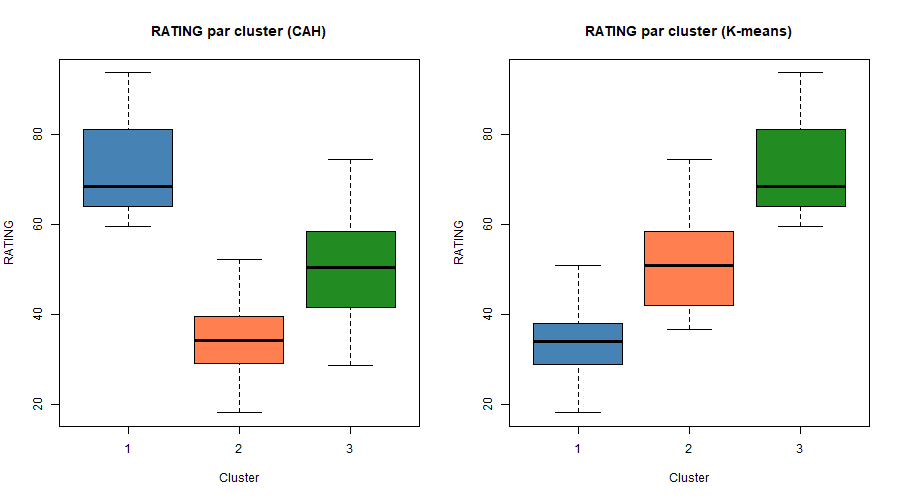
\includegraphics[width=0.6\textwidth]{output/figures/22_rating_par_cluster.png}
\caption{RATING par cluster (CAH à gauche, K-means à droite)}
\end{figure}

Le RATING moyen par profil va dans le même sens : environ 73.8 pour le groupe haute fibre, 51.4 pour le modéré, 33.3 pour le sucré. Sur la figure, à gauche c'est le cluster 1 de la CAH, à droite le cluster 3 du K-means, mais il s'agit du même groupe. La note de Consumer Reports sanctionne le sucre et valorise les fibres, ce qui correspond aux recommandations diététiques courantes.

\section{Conclusion}

L'analyse fait ressortir deux directions de variation. La première est la teneur en fibres, à laquelle le potassium est très lié. La seconde est la densité calorique, portée par les calories, le sucre et le gras. À elles deux, elles expliquent plus de la moitié de la variance.

La classification en 3 groupes, retrouvée de façon cohérente par la CAH et le K-means (Rand = 0.88), distingue les céréales sucrées et caloriques (le plus gros groupe), les céréales modérées et classiques, et une petite niche très riche en fibres, uniquement des All-Bran.

Le résultat le plus parlant concerne RATING. Cette note n'a pas servi à construire les axes, et pourtant elle se place presque exactement le long du gradient fibres / sucre. Consumer Reports note donc la qualité nutritionnelle avec des critères proches de ceux que l'ACP dégage seule.

Reste une limite assumée : à k=3 la silhouette moyenne n'est que de 0.22 et le groupe haute fibre tient sur 3 individus. Un découpage en 2 classes serait statistiquement plus sûr mais effacerait justement ce qui est intéressant. Le test sans les 3 All-Bran a montré que la structure principale ne dépend pas d'eux, ce qui rend le compromis k=3 défendable.

\newpage
\section{Annexe : code R}

Tout le traitement tient dans un seul script, \texttt{scripts/analyse\_cereales.R}, exécutable d'une traite depuis la racine du projet. Packages : FactoMineR, factoextra, corrplot, cluster, moments.

Il enchaîne, dans l'ordre : le prétraitement (recodage des -1 en NA puis imputation médiane), les statistiques univariées et bivariées, l'ACP normée avec variables supplémentaires, la CAH de Ward, le K-means à \texttt{nstart=25}, la comparaison des deux partitions (indice de Rand et pureté) et enfin les projections et le croisement avec RATING. \texttt{set.seed(42)} fixe le tirage du K-means pour que les résultats soient reproductibles.

{\small\verbatiminput{scripts/analyse_cereales.R}}

\end{document}
